\section{Additional Results}
\label{ssec:allresults}

Table~\ref{tab:confintmain} displays the point estimates from all estimators as well as confidence intervals calculated either (a) leave-one-state-out jackknife on the adjusted dataset (CI (states)); (b) leave-one-state-out jackknife repeating the entire adjusted leaving each state out (CI (proc)). This table also includes all analyses calculated on a second version of the adjusted data where we use a common $\kappa$ for all values (sigma\_uu\_avg), which is the adjustment suggested by \cite{carroll2006measurement}. Notice that the confidence intervals are identical for ``sigma\_zero'' because this is the unadjusted dataset. ``sigma\_uu\_i'' is our preferred covariate adjustment.

\begin{table}[ht]
\centering
\caption{Primary point estimates and confidence intervals}
\label{tab:confintmain}
\begin{tabular}{llrll}
  \hline
Weight type & Sigma estimate & Psihat & CI (states) & CI (proc) \\ 
  \hline
H-SBW & sigma\_uu\_i & -2.17 & (-3.41, -0.94) & (-3.42, -0.92) \\ 
  H-SBW & sigma\_uu\_avg & -2.25 & (-3.51, -0.99) & (-3.35, -1.14) \\ 
  H-SBW & sigma\_zero & -2.35 & (-3.09, -1.61) & (-3.09, -1.61) \\ 
  BC-HSBW & sigma\_uu\_i & -2.13 & (-3.55, -0.71) & (-3.16, -1.11) \\ 
  BC-HSBW & sigma\_uu\_avg & -2.17 & (-3.57, -0.78) & (-4.91, 0.56) \\ 
  BC-HSBW & sigma\_zero & -2.40 & (-3.33, -1.46) & (-3.3, -1.49) \\ 
  SBW & sigma\_uu\_i & -2.24 & (-3.50, -0.99) & (-3.51, -0.97) \\ 
  SBW & sigma\_uu\_avg & -2.30 & (-3.67, -0.92) & (-3.45, -1.15) \\ 
  SBW & sigma\_zero & -2.40 & (-3.10, -1.69) & (-3.10, -1.69) \\ 
  BC-SBW & sigma\_uu\_i & -2.12 & (-3.15, -1.10) & (-3.06, -1.19) \\ 
  BC-SBW & sigma\_uu\_avg & -2.17 & (-3.25, -1.08) & (-4.46, 0.12) \\ 
  BC-SBW & sigma\_zero & -2.36 & (-2.93, -1.80) & (-2.88, -1.85) \\ 
   \hline
\end{tabular}
\end{table}

Table ~\ref{tab:deltac1} presents the difference in the estimated contrast when excluding the Republican governance indicators along with inferential estimates. Table~\ref{tab:ptests} presents all point estimates from estimators that we calculated. The ``Var subset`` column indicates which variables were excluded from the estimation: 0 excludes no variables; 1 removes Republican governance indicators; 2 pre-treatment uninsurance and unemployment rates; 3 urban, age, education, citizenship, marital status, student, disability, or female; 4 race, ethnicity, income, foreign born; 5 children, population growth, and household to person ratio. We see that the largest changes generally occur when excluding the pre-treatment uninsurance and unemployment rates. This is not surprising: controlling for the other covariates, the pre-treatment uninsurance rate was substantially lower in the treated region compared to the control region. Given that pre-treatment uninsurance rates are highly correlated with post-treatment rates, we find that this comparison leads to a larger absolute magnitude point estimate, highlighting the need to control for these covariates.

\begin{table}[ht]
\centering
\caption{$\hat{\Delta}^1$ estimates primary dataset}
\label{tab:deltac1}
\begin{tabular}{llrll}
  \hline
Weight type & Sigma estimate & diff & CI state & CI proc \\ 
  \hline
H-SBW & sigma\_uu\_i\_modeled & -0.67 & (-1.63, 0.28) & (-1.66, 0.32) \\ 
  H-SBW & sigma\_uu\_avg & -0.61 & (-1.57, 0.35) & (-1.46, 0.24) \\ 
  H-SBW & sigma\_zero & -0.65 & (-1.20, -0.09) & (-1.2, -0.09) \\ 
  BC-HSBW & sigma\_uu\_i\_modeled & -0.74 & (-1.86, 0.39) & (-1.76, 0.28) \\ 
  BC-HSBW & sigma\_uu\_avg & -0.69 & (-1.79, 0.41) & (-3.62, 2.24) \\ 
  BC-HSBW & sigma\_zero & -0.70 & (-1.48, 0.08) & (-1.53, 0.13) \\ 
  SBW & sigma\_uu\_i\_modeled & -0.75 & (-1.74, 0.24) & (-1.82, 0.31) \\ 
  SBW & sigma\_uu\_avg & -0.70 & (-1.77, 0.38) & (-1.57, 0.17) \\ 
  SBW & sigma\_zero & -0.68 & (-1.28, -0.08) & (-1.28, -0.08) \\ 
  BC-SBW & sigma\_uu\_i\_modeled & -0.63 & (-1.54, 0.28) & (-2.14, 0.88) \\ 
  BC-SBW & sigma\_uu\_avg & -0.58 & (-1.50, 0.34) & (-2.97, 1.81) \\ 
  BC-SBW & sigma\_zero & -0.56 & (-1.13, 0.01) & (-1.1, -0.02) \\ 
   \hline
\end{tabular}
\end{table}

% Wed Jan 13 15:24:43 2021
\begin{table}[ht]
\centering
\caption{Point estimates for all specifications}
\label{tab:ptests}
\begin{tabular}{rlrrrr}
  \toprule
Variable subset & Sigma estimate & H-SBW & BC-HSBW & SBW & BC-SBW \\ 
  \hline
0 & sigma\_uu\_i & -2.17 & -2.13 & -2.24 & -2.12 \\ 
  0 & sigma\_uu\_avg & -2.25 & -2.17 & -2.30 & -2.17 \\ 
  0 & sigma\_zero & -2.35 & -2.40 & -2.40 & -2.36 \\ 
  1 & sigma\_uu\_i & -2.85 & -2.87 & -3.00 & -2.76 \\ 
  1 & sigma\_uu\_avg & -2.86 & -2.86 & -2.99 & -2.75 \\ 
  1 & sigma\_zero & -3.00 & -3.09 & -3.07 & -2.92 \\ 
  2 & sigma\_uu\_i & -5.73 & -5.05 & -5.24 & -4.70 \\ 
  2 & sigma\_uu\_avg & -5.73 & -5.05 & -5.24 & -4.70 \\ 
  2 & sigma\_zero & -5.73 & -5.13 & -5.24 & -4.77 \\ 
  3 & sigma\_uu\_i & -2.17 & -2.00 & -2.24 & -2.00 \\ 
  3 & sigma\_uu\_avg & -2.25 & -2.06 & -2.29 & -2.06 \\ 
  3 & sigma\_zero & -2.34 & -2.17 & -2.40 & -2.15 \\ 
  4 & sigma\_uu\_i & -2.35 & -2.39 & -2.29 & -2.30 \\ 
  4 & sigma\_uu\_avg & -2.39 & -2.39 & -2.32 & -2.32 \\ 
  4 & sigma\_zero & -2.45 & -2.59 & -2.43 & -2.49 \\ 
  5 & sigma\_uu\_i & -2.17 & -2.19 & -2.26 & -2.21 \\ 
  5 & sigma\_uu\_avg & -2.25 & -2.24 & -2.33 & -2.27 \\ 
  5 & sigma\_zero & -2.35 & -2.44 & -2.42 & -2.47 \\ 
   \hline
\end{tabular}
\end{table}

Table ~\ref{tab:confintmainc2}, Table~\ref{tab:deltac2}, and Table~\ref{tab:secondaryptests} are identical to the structure of the previous two tables except we exclude the ``early expansion states'' from the pool of expansion state matches. 

\begin{table}[ht]
\centering
\caption{Early expansion excluded, point estimates and confidence intervals}
\label{tab:confintmainc2}
\begin{tabular}{llrll}
  \toprule
Weight type & Sigma estimate & Psihat & CI (states) & CI (proc) \\ 
  \midrule
H-SBW & sigma\_uu\_i & -2.05 & (-3.10, -1.00) & (-3.05, -1.05) \\ 
  H-SBW & sigma\_uu\_avg & -2.13 & (-3.20, -1.05) & (-3.17, -1.08) \\ 
  H-SBW & sigma\_zero & -2.29 & (-2.90, -1.69) & (-2.90, -1.69) \\ 
  BC-HSBW & sigma\_uu\_i & -2.14 & (-3.63, -0.64) & (-3.45, -0.82) \\ 
  BC-HSBW & sigma\_uu\_avg & -2.19 & (-3.65, -0.73) & (-3.79, -0.59) \\ 
  BC-HSBW & sigma\_zero & -2.50 & (-3.66, -1.33) & (-3.69, -1.31) \\ 
  SBW & sigma\_uu\_i & -1.91 & (-2.91, -0.91) & (-2.79, -1.03) \\ 
  SBW & sigma\_uu\_avg & -2.01 & (-3.02, -1.00) & (-2.83, -1.19) \\ 
  SBW & sigma\_zero & -2.20 & (-2.69, -1.71) & (-2.69, -1.71) \\ 
  BC-SBW & sigma\_uu\_i & -1.97 & (-3.49, -0.44) & (-3.53, -0.40) \\ 
  BC-SBW & sigma\_uu\_avg & -2.04 & (-3.59, -0.50) & (-3.44, -0.65) \\ 
  BC-SBW & sigma\_zero & -2.34 & (-3.44, -1.25) & (-3.46, -1.23) \\ 
   \bottomrule
\end{tabular}
\end{table}

\begin{table}[ht]
\centering
\caption{$\hat{\Delta}^1$ estimates, early expansion excluded}
\label{tab:deltac2}
\begin{tabular}{llrll}
  \toprule
Weight type & Sigma estimate & diff & CI state & CI proc \\ 
  \midrule
H-SBW & sigma\_uu\_i\_modeled & -0.80 & (-1.69, 0.09) & (-1.62, 0.02) \\ 
  H-SBW & sigma\_uu\_avg & -0.73 & (-1.68, 0.22) & (-1.57, 0.11) \\ 
  H-SBW & sigma\_zero & -0.76 & (-1.52, -0.01) & (-1.52, -0.01) \\ 
  BC-HSBW & sigma\_uu\_i\_modeled & -0.85 & (-2.16, 0.46) & (-2.15, 0.45) \\
  BC-HSBW & sigma\_uu\_avg & -0.79 & (-2.08, 0.49) & (-2.16, 0.57) \\ 
  BC-HSBW & sigma\_zero & -0.69 & (-1.9, 0.52) & (-2.02, 0.65) \\ 
  SBW & sigma\_uu\_i\_modeled & -0.94 & (-1.73, -0.15) & (-1.61, -0.27) \\ 
  SBW & sigma\_uu\_avg & -0.85 & (-1.62, -0.08) & (-1.39, -0.31) \\ 
  SBW & sigma\_zero & -0.76 & (-1.51, -0.01) & (-1.51, -0.01) \\ 
  BC-SBW & sigma\_uu\_i\_modeled & -0.89 & (-2.41, 0.62) & (-2.58, 0.79) \\ 
  BC-SBW & sigma\_uu\_avg & -0.82 & (-2.36, 0.72) & (-1.96, 0.33) \\ 
  BC-SBW & sigma\_zero & -0.64 & (-1.86, 0.57) & (-2.21, 0.93) \\ 
   \bottomrule
\end{tabular}
\end{table}

\begin{table}[ht]
\centering
   \caption{Point estimates for all specifications, early expansion excluded}
    \label{tab:secondaryptests}
\begin{tabular}{rlrrrr}
  \hline
Variable subset & Sigma estimate & H-SBW & BC-HSBW & SBW & BC-SBW \\ 
  \hline
0 & sigma\_uu\_i & -2.05 & -2.14 & -1.91 & -1.97 \\ 
  0 & sigma\_uu\_avg & -2.13 & -2.19 & -2.01 & -2.04 \\ 
  0 & sigma\_zero & -2.29 & -2.50 & -2.20 & -2.34 \\ 
  1 & sigma\_uu\_i & -2.85 & -2.99 & -2.85 & -2.86 \\ 
  1 & sigma\_uu\_avg & -2.86 & -2.98 & -2.86 & -2.86 \\ 
  1 & sigma\_zero & -3.05 & -3.18 & -2.96 & -2.99 \\ 
  2 & sigma\_uu\_i & -5.55 & -4.46 & -5.02 & -4.52 \\ 
  2 & sigma\_uu\_avg & -5.55 & -4.73 & -5.01 & -4.53 \\ 
  2 & sigma\_zero & -5.55 & -4.78 & -5.01 & -4.56 \\ 
  3 & sigma\_uu\_i & -2.05 & -2.03 & -1.91 & -1.89 \\ 
  3 & sigma\_uu\_avg & -2.13 & -2.10 & -2.00 & -1.97 \\ 
  3 & sigma\_zero & -2.27 & -2.22 & -2.20 & -2.13 \\ 
  4 & sigma\_uu\_i & -2.27 & -2.24 & -2.15 & -2.00 \\ 
  4 & sigma\_uu\_avg & -2.35 & -2.28 & -2.23 & -2.04 \\ 
  4 & sigma\_zero & -2.36 & -2.62 & -2.28 & -2.45 \\ 
  5 & sigma\_uu\_i & -2.05 & -2.20 & -1.91 & -2.03 \\ 
  5 & sigma\_uu\_avg & -2.13 & -2.26 & -1.99 & -2.11 \\ 
  5 & sigma\_zero & -2.29 & -2.45 & -2.19 & -2.36 \\ 
   \hline
\end{tabular}
\end{table}

Table~\ref{tab:loostatec1} and Table~\ref{tab:loostatec2} present point estimates for the leave-one-state out analysis for our preferred estimator, H-SBW calculated on our preferred covariate adjustment for the primary dataset and when excluding early expansion states.

\begin{table}[ht]
\centering
   \caption{Leave-one-state-out point estimates, primary dataset, preferred adjustment}
    \label{tab:loostatec1}
\begin{tabular}{lrlrl}
  \hline
State & Psihat (0) & None (states, proc) & Psihat (1) & Repub (states, proc) \\ 
  \hline
AR & -2.17 & (-2.34, -2.38) & -2.85 & (-2.81, -2.80) \\ 
  AZ & -2.17 & (-2.21, -2.24) & -2.85 & (-2.86, -2.86) \\ 
  CA & -2.17 & (-1.99, -2.02) & -2.85 & (-2.77, -2.76) \\ 
  CO & -2.17 & (-2.17, -2.23) & -2.85 & (-2.84, -2.84) \\ 
  CT & -2.17 & (-2.17, -2.15) & -2.85 & (-2.83, -2.82) \\ 
  HI & -2.17 & (-2.15, -2.14) & -2.85 & (-2.77, -2.78) \\ 
  IA & -2.17 & (-2.09, -2.07) & -2.85 & (-2.83, -2.84) \\ 
  IL & -2.17 & (-2.16, -2.24) & -2.85 & (-2.83, -2.84) \\ 
  KY & -2.17 & (-2.02, -1.95) & -2.85 & (-2.57, -2.52) \\ 
  MD & -2.17 & (-2.25, -2.27) & -2.85 & (-2.94, -2.94) \\ 
  MI & -2.17 & (-2.10, -2.18) & -2.85 & (-2.89, -2.92) \\ 
  MN & -2.17 & (-2.17, -2.19) & -2.85 & (-2.84, -2.86) \\ 
  ND & -2.17 & (-2.23, -2.26) & -2.85 & (-2.84, -2.84) \\ 
  NH & -2.17 & (-2.18, -2.21) & -2.85 & (-2.98, -2.99) \\ 
  NJ & -2.17 & (-2.26, -2.25) & -2.85 & (-2.99, -3.03) \\ 
  NM & -2.17 & (-2.16, -2.22) & -2.85 & (-2.76, -2.77) \\ 
  NV & -2.17 & (-2.21, -2.24) & -2.85 & (-2.89, -2.88) \\ 
  OH & -2.17 & (-2.70, -2.68) & -2.85 & (-3.00, -2.98) \\ 
  OR & -2.17 & (-2.17, -2.25) & -2.85 & (-2.80, -2.84) \\ 
  RI & -2.17 & (-2.17, -2.15) & -2.85 & (-2.81, -2.81) \\ 
  WA & -2.17 & (-2.10, -2.11) & -2.85 & (-2.78, -2.77) \\ 
  WV & -2.17 & (-2.16, -2.18) & -2.85 & (-2.80, -2.78) \\ 
   \hline
\end{tabular}
\end{table}

\begin{table}[ht]
\centering
   \caption{Leave-one-state-out point estimates, early expansion excluded, preferred adjustment}
    \label{tab:loostatec2}
\begin{tabular}{lrlrl}
  \toprule
State & Psihat (0) & None (states, proc) & Psihat (1) & Repub (states, proc) \\ 
  \midrule
AR & -2.05 & (-2.15, -2.16) & -2.85 & (-2.77, -2.76) \\ 
  AZ & -2.05 & (-1.82, -1.88) & -2.85 & (-2.87, -2.86) \\ 
  CO & -2.05 & (-2.07, -2.09) & -2.85 & (-2.84, -2.83) \\ 
  HI & -2.05 & (-2.01, -1.99) & -2.85 & (-2.71, -2.73) \\ 
  IA & -2.05 & (-1.98, -1.95) & -2.85 & (-2.85, -2.86) \\ 
  IL & -2.05 & (-2.03, -2.01) & -2.85 & (-2.8, -2.79) \\ 
  KY & -2.05 & (-1.87, -1.80) & -2.85 & (-2.59, -2.54) \\ 
  MD & -2.05 & (-2.18, -2.15) & -2.85 & (-2.97, -2.96) \\ 
  MI & -2.05 & (-1.96, -2.00) & -2.85 & (-2.92, -2.96) \\ 
  ND & -2.05 & (-2.02, -2.04) & -2.85 & (-2.84, -2.84) \\ 
  NH & -2.05 & (-2.05, -2.06) & -2.85 & (-3.02, -3.03) \\ 
  NM & -2.05 & (-1.99, -1.97) & -2.85 & (-2.72, -2.75) \\ 
  NV & -2.05 & (-2.15, -2.15) & -2.85 & (-2.93, -2.92) \\ 
  OH & -2.05 & (-2.43, -2.38) & -2.85 & (-3.03, -3.02) \\ 
  OR & -2.05 & (-2.05, -2.11) & -2.85 & (-2.81, -2.84) \\ 
  RI & -2.05 & (-2.05, -2.05) & -2.85 & (-2.80, -2.80) \\ 
  WV & -2.05 & (-2.06, -2.06) & -2.85 & (-2.83, -2.81) \\ 
   \bottomrule
\end{tabular}
\end{table}

Finally, Figure~\ref{fig:rdiffc1state}, Figure~\ref{fig:rdiffc1proc}, Figure~\ref{fig:rdiffc2state}, and Figure~\ref{fig:rdiffc2proc} display heatmaps showing the estimates of $\hat{\Delta}$ for all of our estimators when removing each state. We see that these estimates are overwhelmingly negative. We only estimate positive contrasts on our primary dataset when recalculating the covariate adjustment excluding that state and when the estimator could extrapolate beyond the support of the data. For the primary dataset, this occurred with California and Illinois. When removing early expansion states this only occurred when removing Hawaii and Ohio for our less preferred covariate adjustment.

We also caution against over-interpreting those particular estimates: as we noted in Appendix C, the covariate adjustments can result in estimates that are outside of the support of the data, or even possible values. While quite rare on our primary dataset, these bad estimates occur more frequently when we recalculate the adjustment when removing each state. In general, we expect estimators that do not extrapolate to be less affected by these bad adjustments, since they will likely get close to no weight; however, estimators that extrapolate are more likely to use the data from these CPUMAs, resulting in dubious estimates. 

\begin{figure}[]
\begin{center}
    \caption{$\hat{\Delta}$ leave-one-out state, primary dataset, covariate adjustment constant}
    \label{fig:rdiffc1state}
    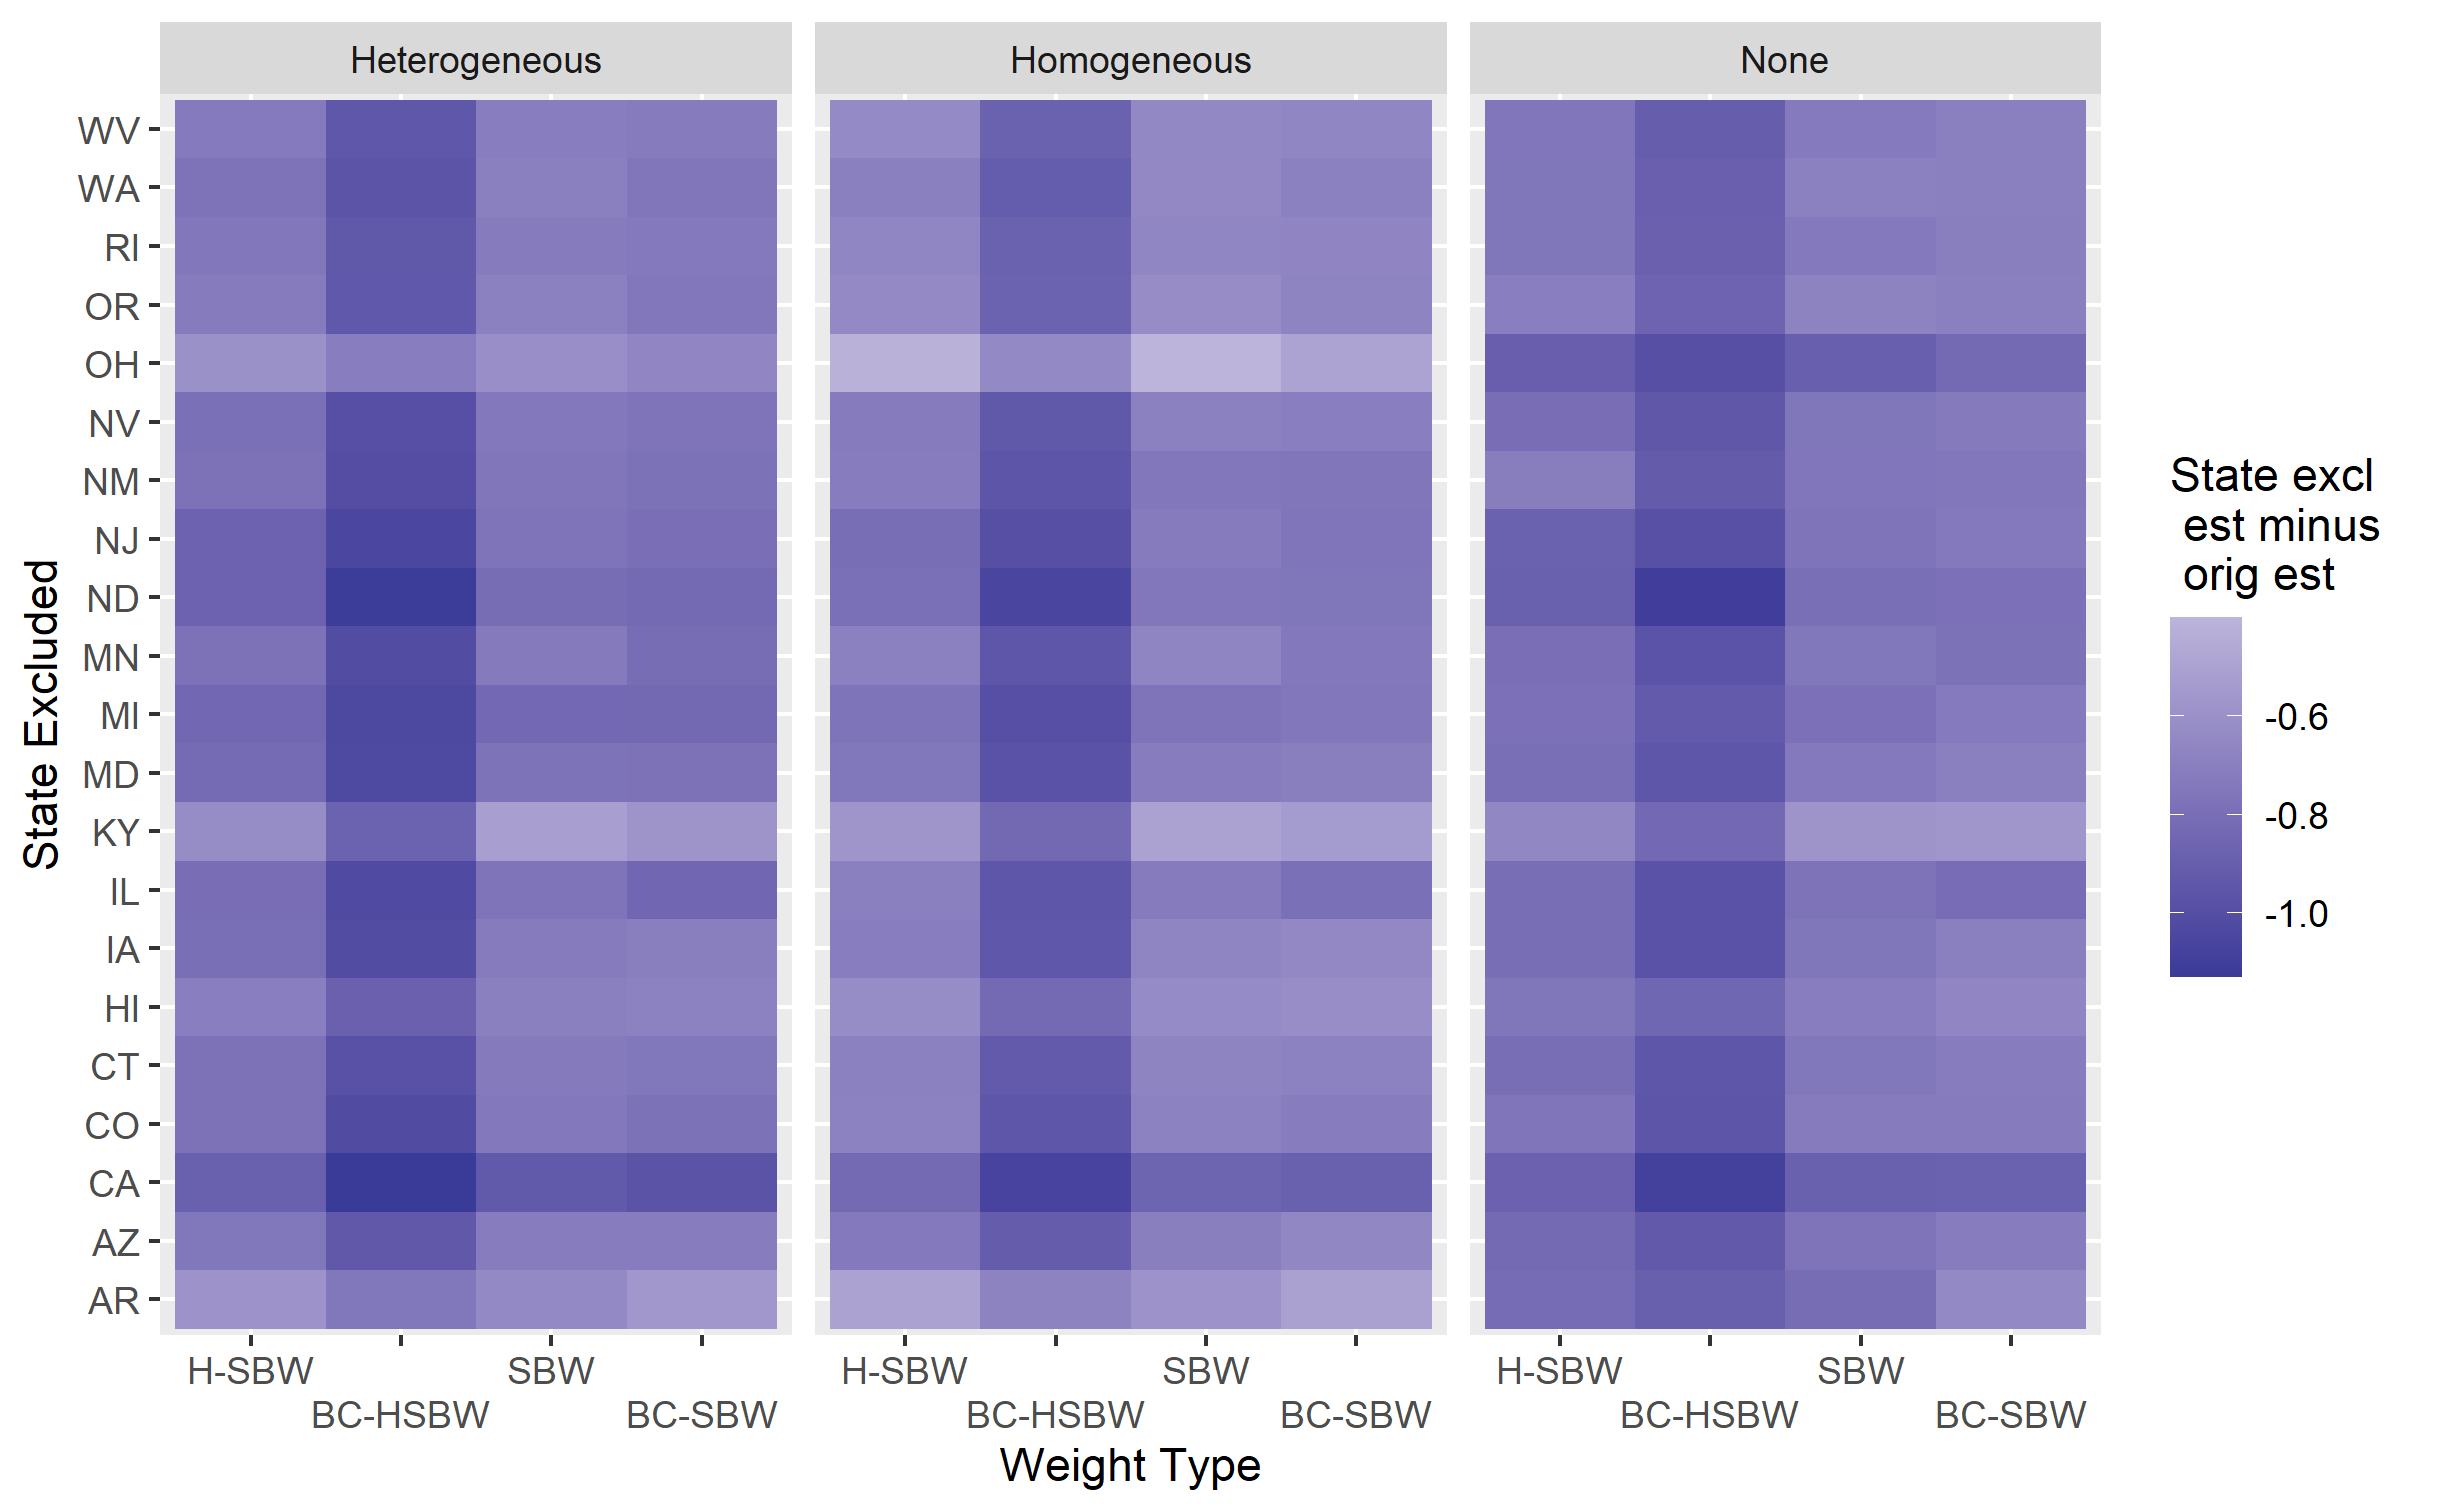
\includegraphics[scale=0.6]{01_Plots/loostate-repub-sensitivityc1-state-main.png}
\end{center}
\end{figure}

\begin{figure}[]
\begin{center}
    \caption{$\hat{\Delta}$ leave-one-out state, primary dataset, covariate adjustment recalculated}
    \label{fig:rdiffc1proc}
    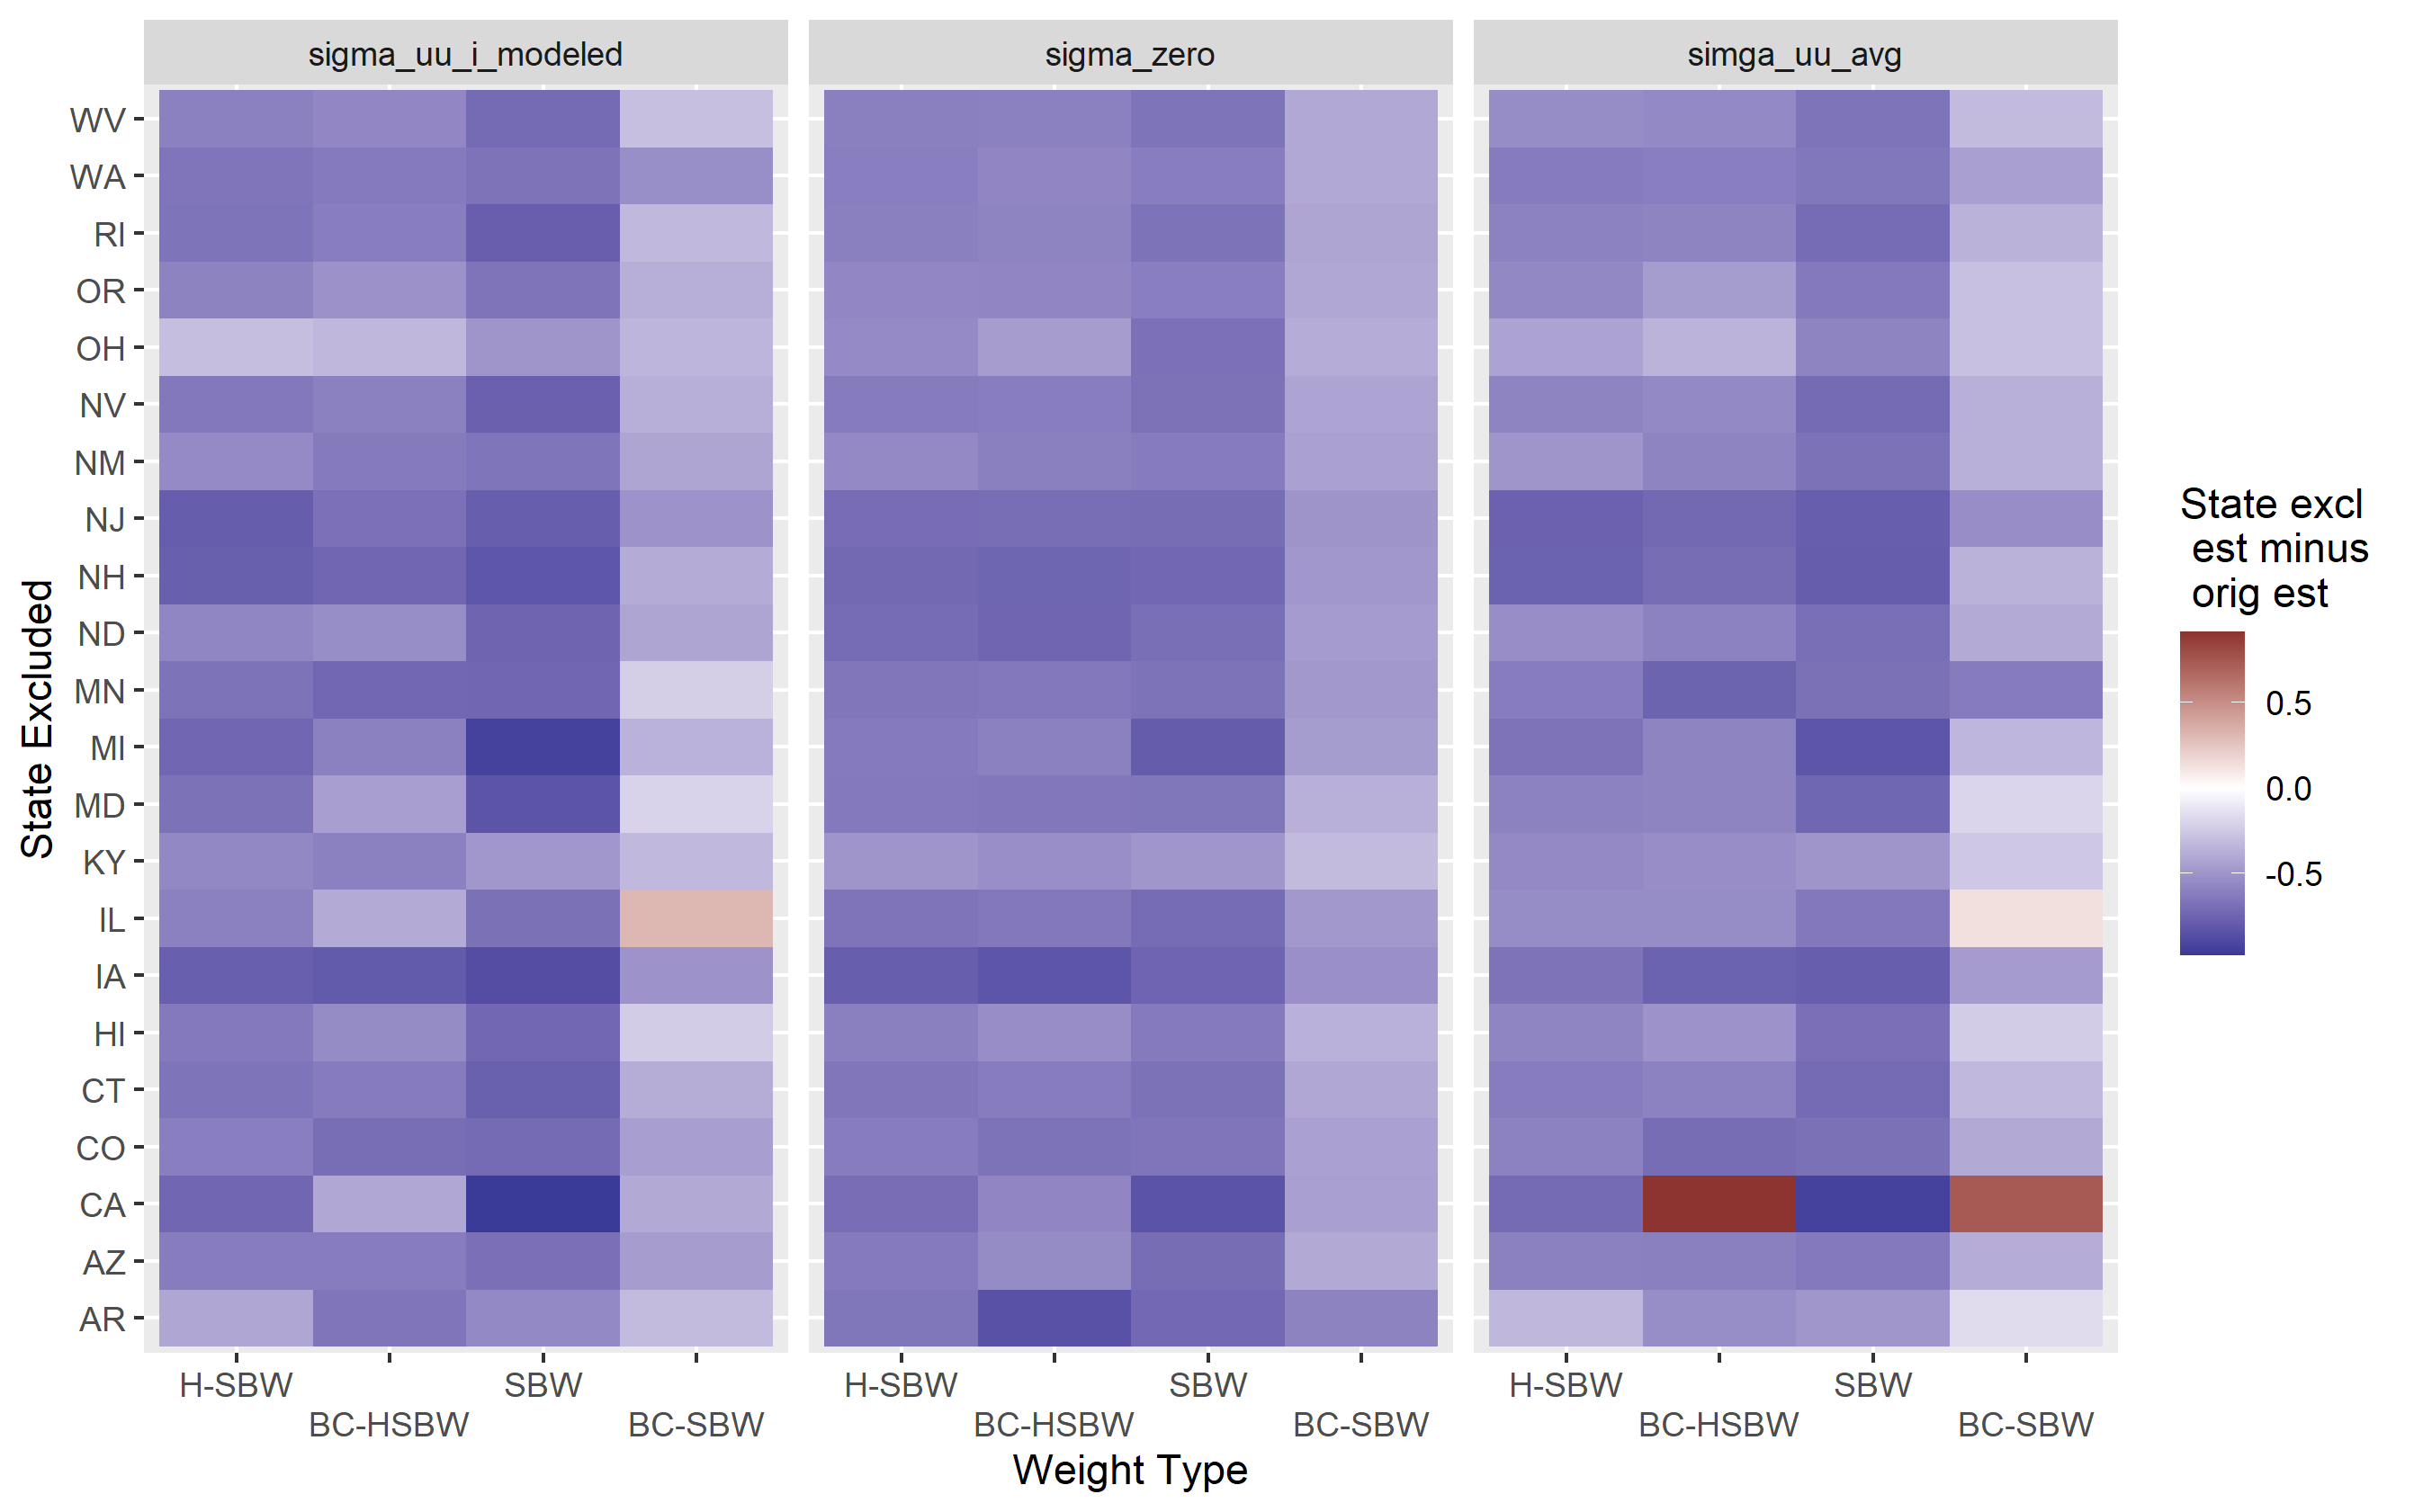
\includegraphics[scale=0.6]{01_Plots/loostate-repub-sensitivityc1-proc-main.png}
\end{center}
\end{figure}

\begin{figure}[]
\begin{center}
    \caption{$\hat{\Delta}$ leave-one-out state, early expansion excluded, covariate adjustment constant}
    \label{fig:rdiffc2state}
    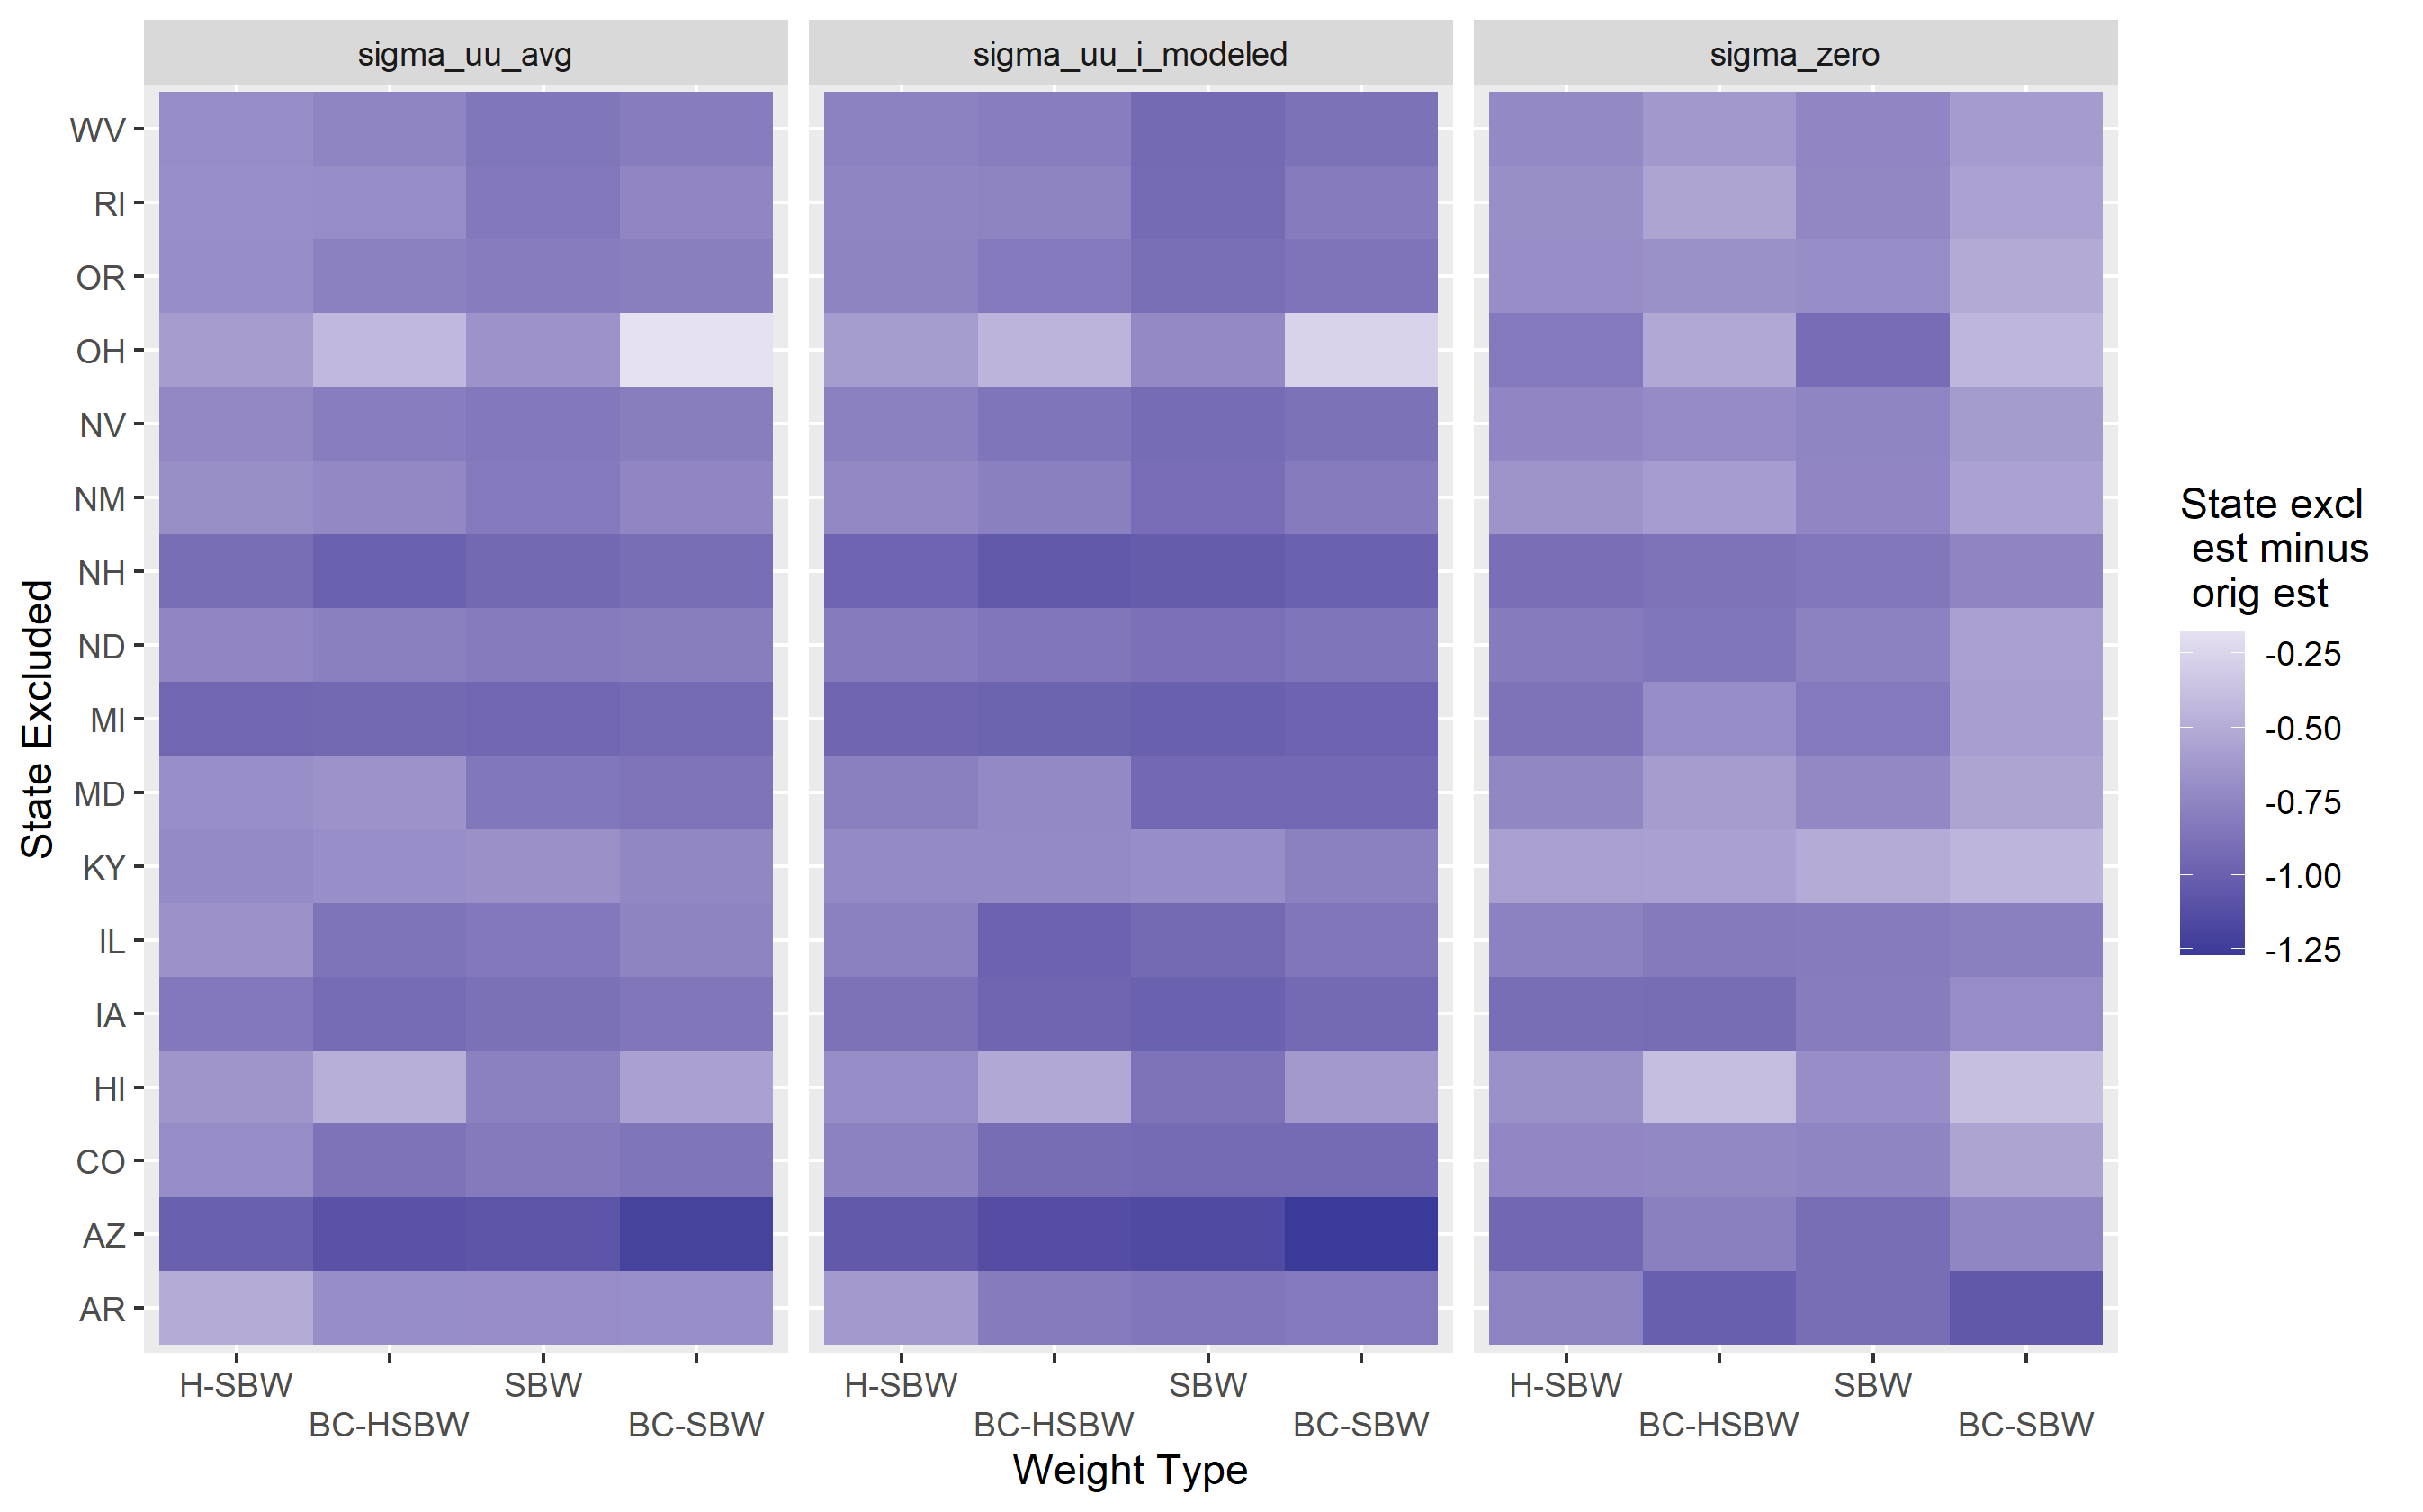
\includegraphics[scale=0.6]{01_Plots/loostate-repub-sensitivityc2-state-main.png}
\end{center}
\end{figure}

\begin{figure}[]
\begin{center}
    \caption{$\hat{\Delta}$ leave-one-out state, early expansion excluded, covariate adjustment recalculated}
    \label{fig:rdiffc2proc}
    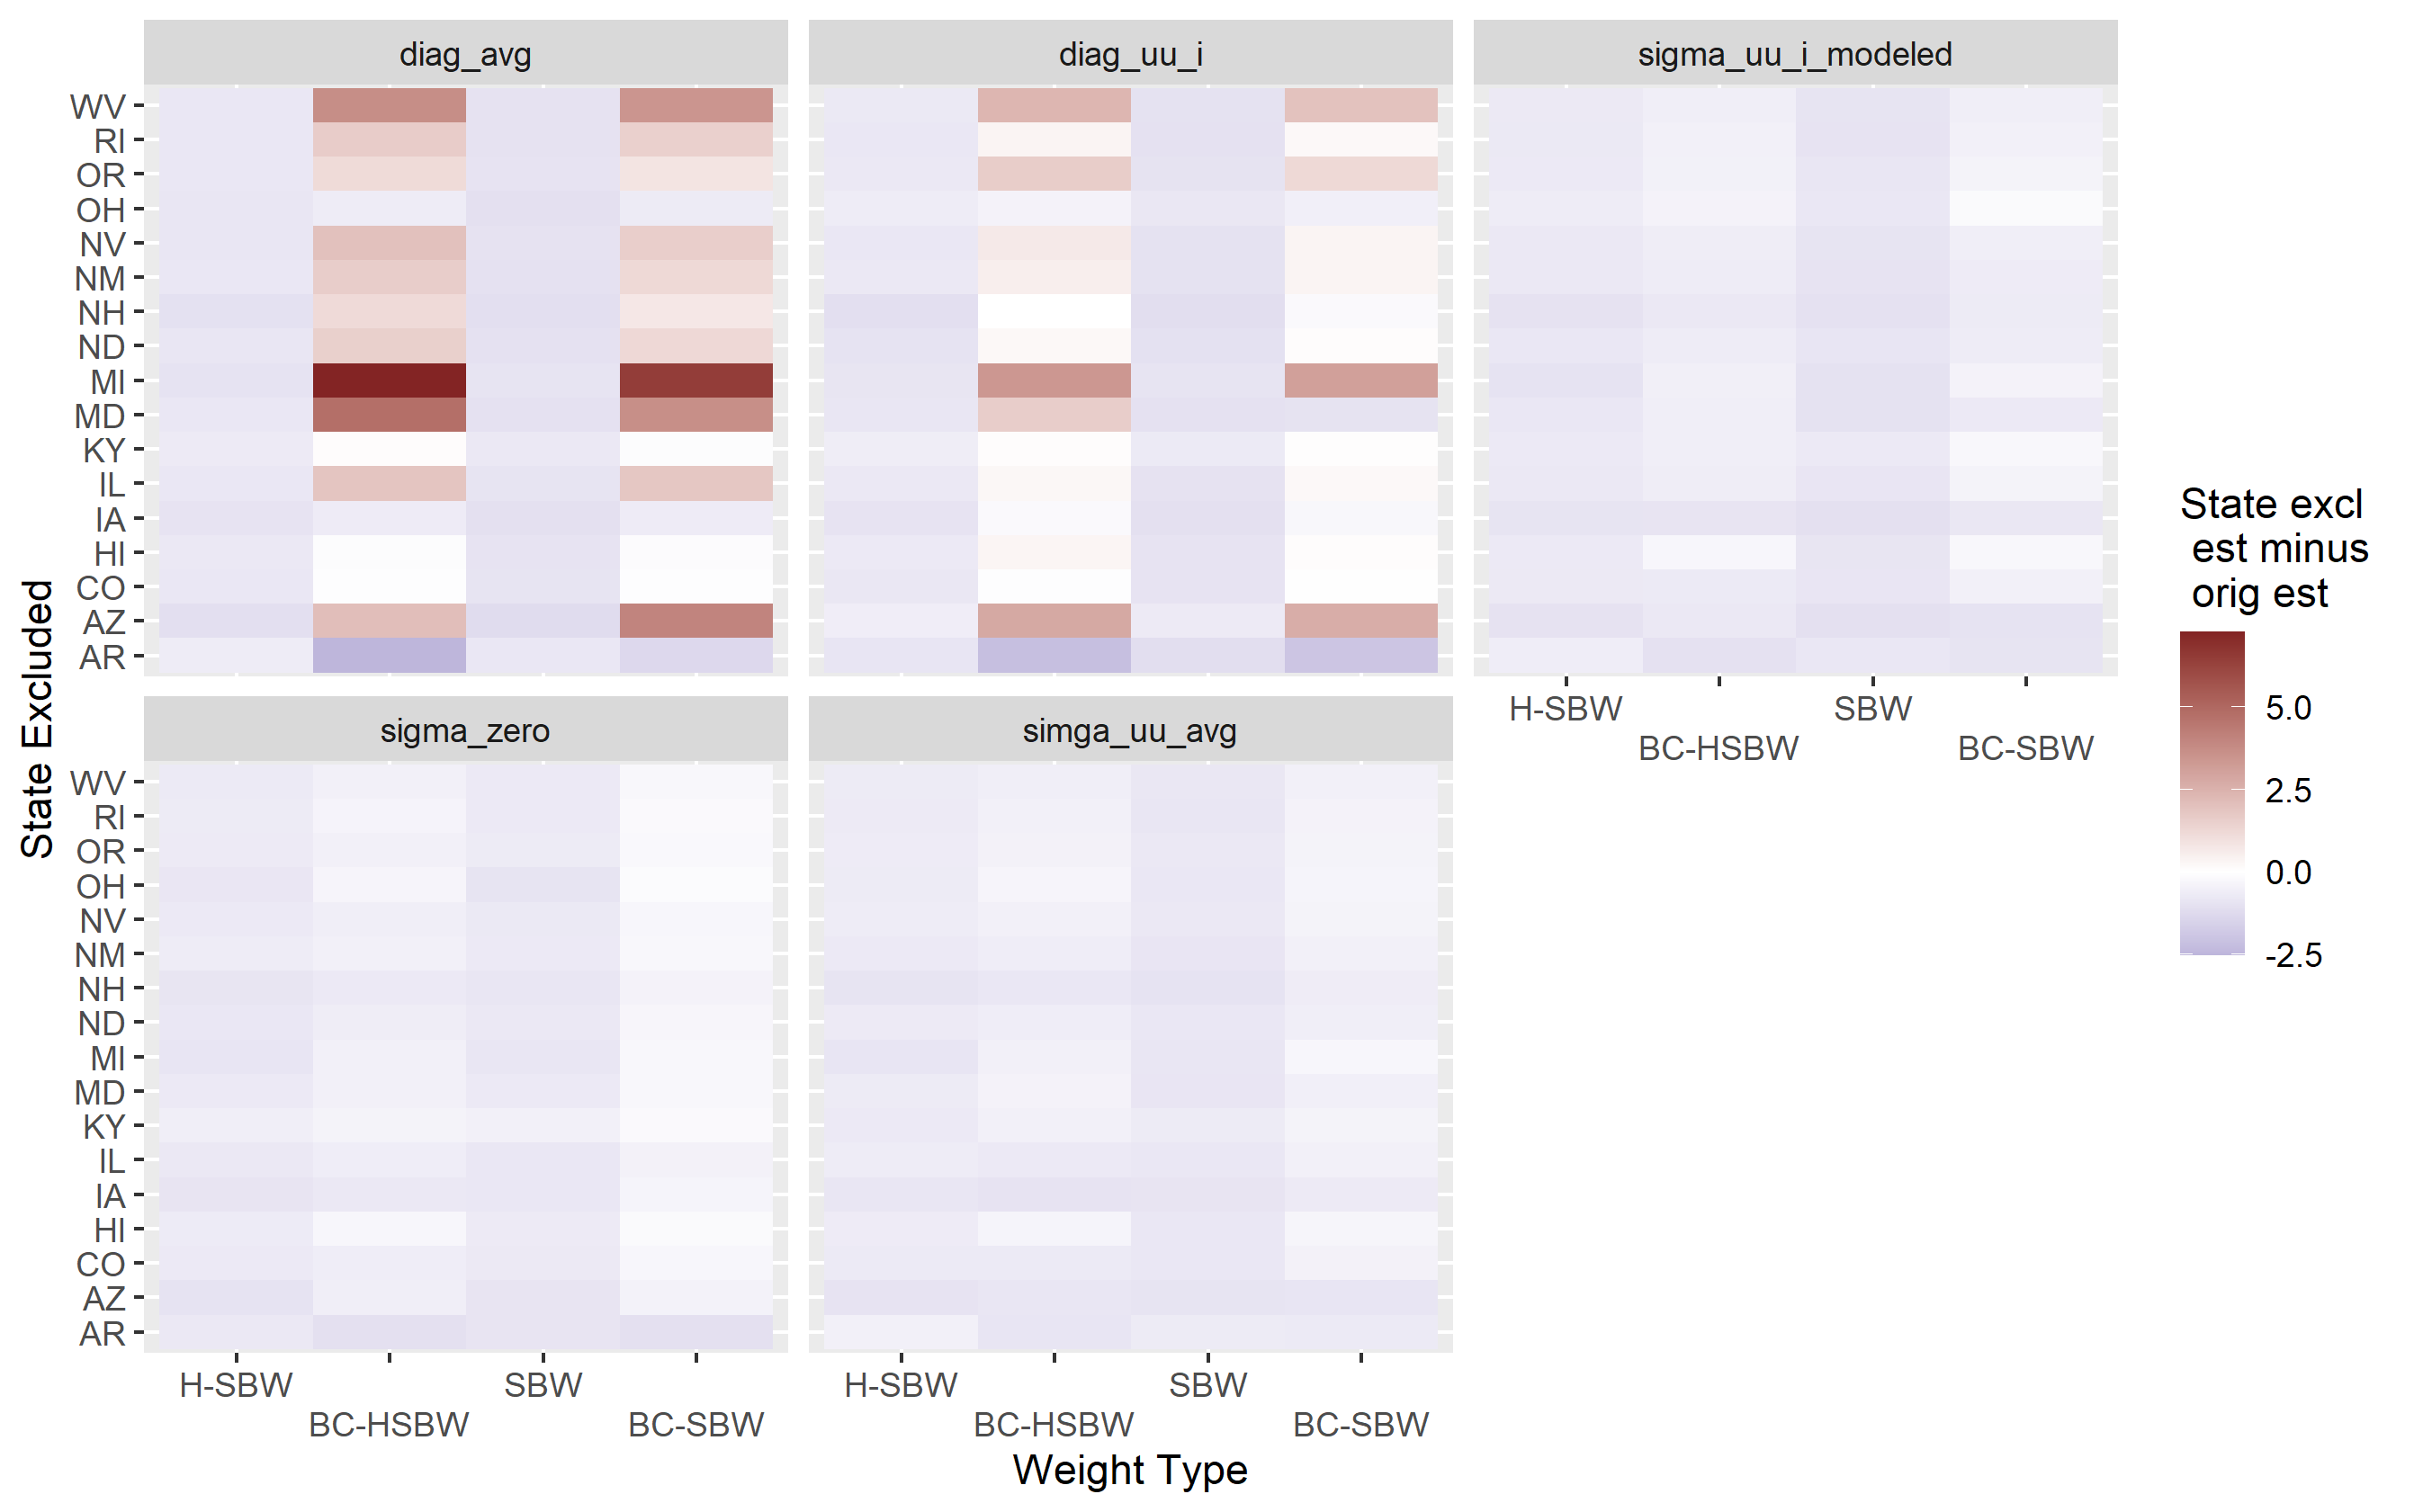
\includegraphics[scale=0.6]{01_Plots/loostate-repub-sensitivityc2-proc-main.png}
\end{center}
\end{figure}

Table~\ref{tab:oateconfint} displays point estimates and confidence intervals for the primary point estimates for the OATE. We display the confidence intervals calculated using both the leave-one-out-states conditional on the covariate adjustment (CI (states)) and recalculating the covariate adjustment for the OATE (CI (proc)). 

\begin{table}[ht]
\centering
\caption{OATE primary results inference}
\label{tab:oateconfint}
\begin{tabular}{rllll}
  \hline
Psihat & Sigma estimate & Dataset & CI (states) & CI (proc) \\ 
  \hline
-1.74 & sigma\_uu\_i\_modeled & c1 & (-2.35, -1.14) & (-2.48, -1.00) \\ 
  -1.67 & sigma\_uu\_avg & c1 & (-2.34, -0.99) & (-2.52, -0.81) \\ 
  -1.80 & sigma\_zero & c1 & (-2.50, -1.10) & (-2.50, -1.10) \\ 
  -1.89 & sigma\_uu\_i\_modeled & c2 & (-2.47, -1.32) & (-2.54, -1.24) \\ 
  -1.80 & sigma\_uu\_avg & c2 & (-2.43, -1.17) & (-2.57, -1.03) \\ 
  -1.95 & sigma\_zero & c2 & (-2.65, -1.25) & (-2.65, -1.25) \\ 
   \hline
\end{tabular}
\end{table}

Table~\ref{tab:oaterepubdiff} displays the difference between the estimated contrasts when excluding Republican governance indicators and when including all covariates as well as the estimated confidence intervals, estimated both conditional on the imputation (CI (states)) and recalculating the entire covariate adjustment (CI (proc)).

\begin{table}[ht]
\centering
\caption{OATE $\hat{\Delta}$ estimates}
\label{tab:oaterepubdiff}
\begin{tabular}{llrll}
  \hline
Sigma estimate & Dataset & Difference & CI (states) & CI (proc) \\ 
  \hline
sigma\_uu\_i\_modeled & c1 & -0.90 & (-1.09, -0.70) & (-1.12, -0.67) \\ 
  sigma\_uu\_i\_modeled & c2 & -0.65 & (-0.86, -0.43) & (-0.88, -0.42) \\ 
  sigma\_uu\_avg & c1 & -0.94 & (-1.15, -0.72) & (-1.20, -0.67) \\ 
  sigma\_uu\_avg & c2 & -0.67 & (-0.90, -0.44) & (-0.91, -0.43) \\ 
  sigma\_zero & c1 & -0.76 & (-0.93, -0.58) & (-0.93, -0.58) \\ 
  sigma\_zero & c2 & -0.56 & (-0.75, -0.38) & (-0.75, -0.38) \\ 
   \hline
\end{tabular}
\end{table}

Table~\ref{tab:oatesensitive} presents all point estimates calculate using the overlap weights. Dataset ``c1'' refers to the primary dataset and dataset ``c2'' removes the early expansion states. The numeric column names refer to the covariate group excluded (covariate groups described above).

\begin{table}[ht]
\centering
\caption{OATE all point estimates}
\label{tab:oatesensitive}
\begin{tabular}{llrrrrrr}
  \hline
Sigma estimate & Dataset & 0 & 1 & 2 & 3 & 4 & 5 \\ 
  \hline
sigma\_uu\_i & c1 & -1.64 & -2.60 & -2.96 & -1.86 & -1.86 & -1.77 \\ 
  sigma\_uu\_i & c2 & -1.81 & -2.53 & -3.10 & -2.18 & -2.04 & -1.96 \\ 
  sigma\_avg & c1 & -1.58 & -2.62 & -2.85 & -1.76 & -1.76 & -1.78 \\ 
  sigma\_avg & c2 & -1.74 & -2.54 & -3.00 & -2.10 & -1.96 & -1.95 \\ 
  sigma\_zero & c1 & -1.80 & -2.55 & -3.11 & -1.98 & -1.94 & -1.83 \\ 
  sigma\_zero & c2 & -1.95 & -2.51 & -3.25 & -2.12 & -2.10 & -2.00 \\ 
   \hline
\end{tabular}
\end{table}

Figure~\ref{fig:oateheatmap} displays a heatmap showing how the OATE point estimates change when removing each state, conditional on our preferred covariate adjustment for both the primary dataset and when excluding early expansion states. We present the results for all covariates and excluding the Republican governance indicators. Additional results are available on request. We see that our point estimates move closer to zero when removing Wisconsin or Ohio for all specifications. Removing Arkansas appears to generally move the point estimates further away from zero.

\begin{figure}[]
\begin{center}
    \caption{OATE estimates, leave-one-out-states analysis}
    \label{fig:oateheatmap}
    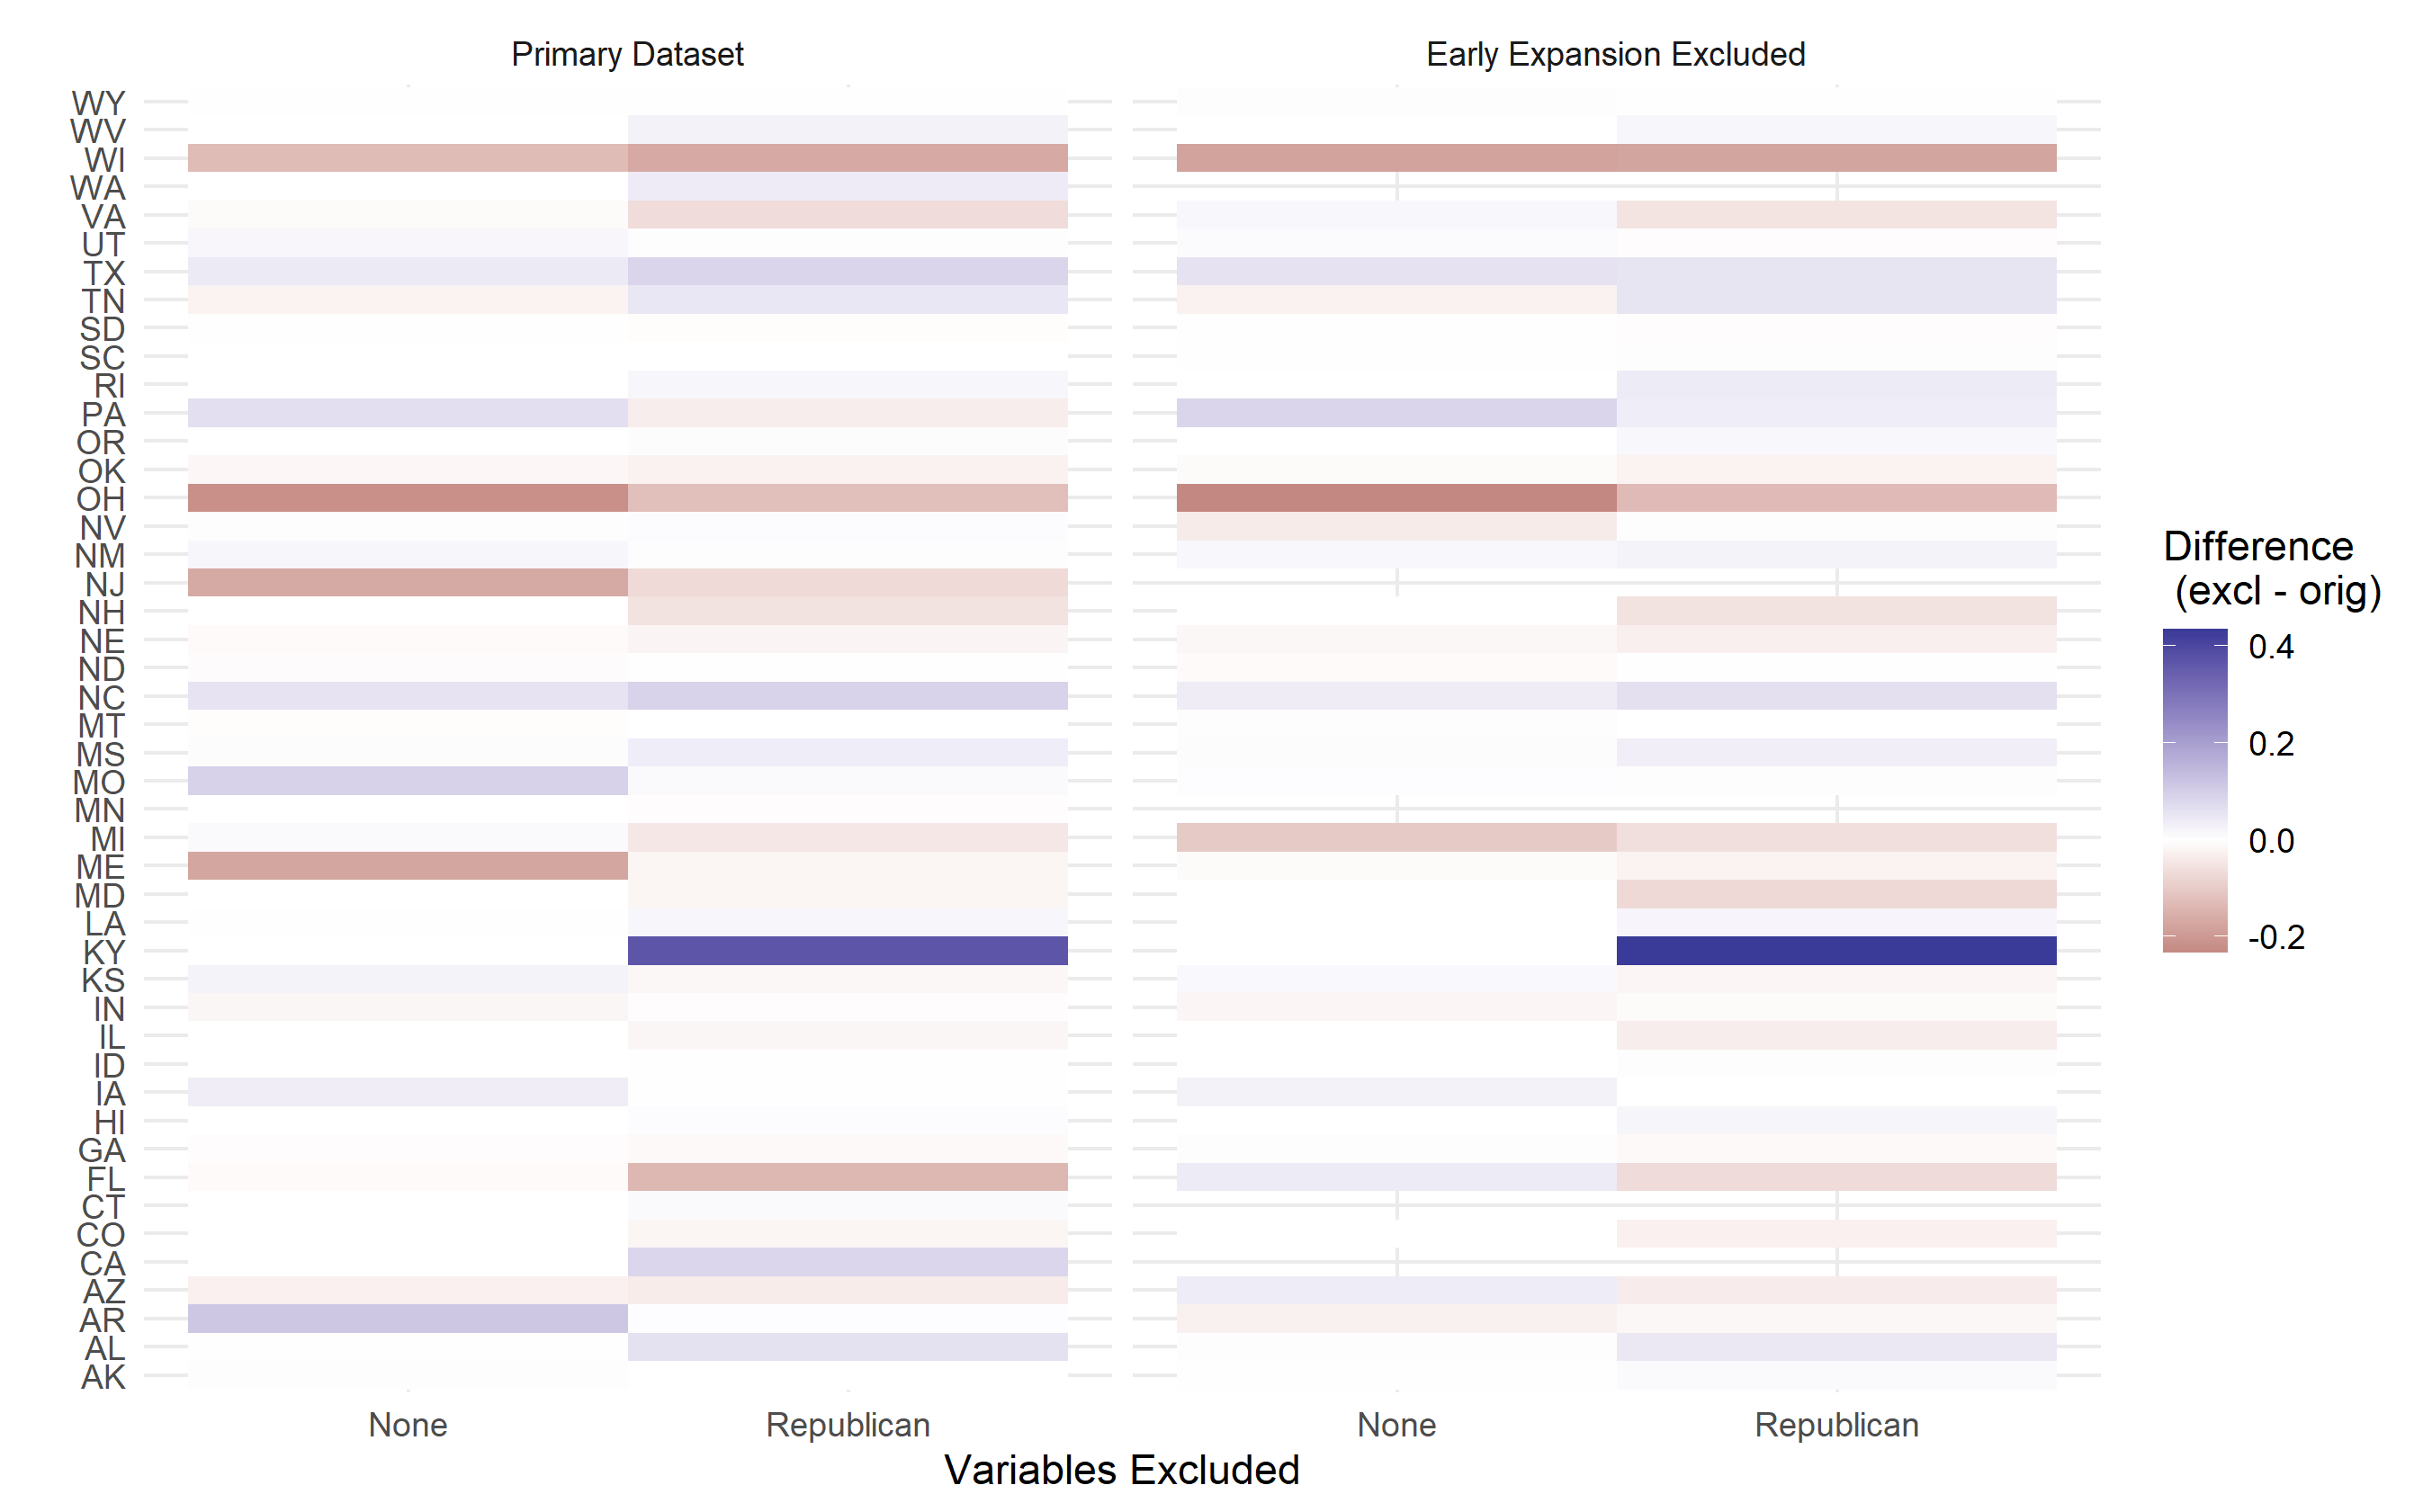
\includegraphics[scale=0.6]{01_Plots/oate-loo-state-cov-group-heatmap-states.png}
\end{center}
\end{figure}
